\documentclass[tikz,border=0pt,crop=true]{standalone}

\usepackage{tikz} % Allows creation of tikz pictures
\usepackage{varwidth}
\usetikzlibrary{arrows,shapes}

\begin{document}
    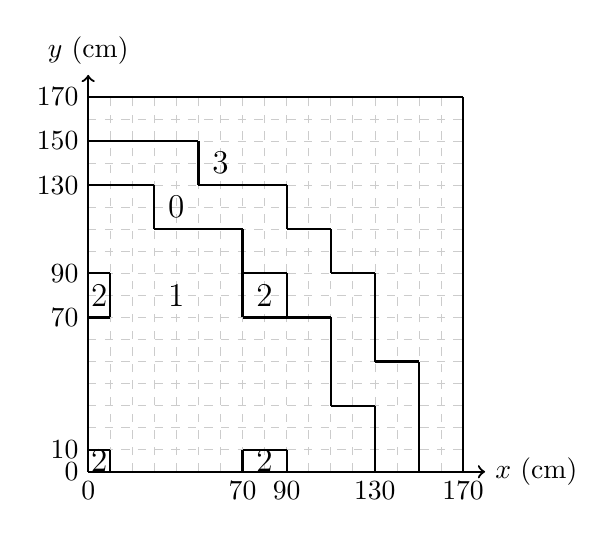
\begin{tikzpicture}[scale=.28]
    \begin{scope}<->;
        % GRID
        \draw[step=1.0,gray,very thin, dashed,opacity=0.4] (0.0,0.0) grid (17.0, 17.0); 
        
        % AXES
        \draw[black, thick, ->] (0, 0) -- (18,  0) node[right] {$x$ (cm)};
        \draw[black, thick, ->] (0, 0) -- ( 0, 18) node[above] {$y$ (cm)};
        
        % Material 3 regions
        \draw[black, thick] (  0.0, 17.0) -- (17.0, 17.0);
        \draw[black, thick] (  17.0, 17.0) -- (17.0, 0.0);  
        \node[font=\large] at (6.0, 14.0) {3};
        
        % Material 0 regions
        \draw[black, thick] (  0.0, 15.0) -- (5.0, 15.0);
        \draw[black, thick] (  5.0, 15.0) -- (5.0, 13.0);  
        \draw[black, thick] (  5.0, 13.0) -- (9.0, 13.0);
        \draw[black, thick] (  9.0, 13.0) -- (9.0, 11.0);
        \draw[black, thick] (  9.0, 11.0) -- (11.0, 11.0); 
        \draw[black, thick] (  11.0, 11.0) -- (11.0, 9.0); 
        \draw[black, thick] (  11.0, 9.0) -- (13.0, 9.0); 
        \draw[black, thick] (  13.0, 9.0) -- (13.0, 5.0);
        \draw[black, thick] (  15.0, 5.0) -- (13.0, 5.0);
        \draw[black, thick] (  15.0, 5.0) -- (15.0, 0.0);
        \node[font=\large] at (4.0, 12.0) {0};
        
        % Material 1 regions
        \draw[black, thick] (  0.0, 13.0) -- (3.0, 13.0);
        \draw[black, thick] (  3.0, 13.0) -- (3.0, 11.0);  
        \draw[black, thick] (  3.0, 11.0) -- (7.0, 11.0);
        \draw[black, thick] (  7.0, 11.0) -- (7.0, 7.0);
        \draw[black, thick] (  7.0, 7.0) -- (11.0, 7.0); 
        \draw[black, thick] (  11.0, 7.0) -- (11.0, 3.0);  
        \draw[black, thick] (  11.0, 3.0) -- (13.0, 3.0);  
        \draw[black, thick] (  13.0, 3.0) -- (13.0, 0.0);  
        \node[font=\large] at (4.0, 8.0) {1};
        
        % Material 2 regions
        \draw[black, thick] (  0.0, 0.0) -- (0.0, 1.0);
        \draw[black, thick] (  1.0, 1.0) -- (1.0, 0.0);  
        \draw[black, thick] (  0.0, 1.0) -- (1.0, 1.0);
        \node[font=\large] at (0.5, 0.5) {2};  
        
        \draw[black, thick] (  0.0, 7.0) -- (1.0, 7.0); 
        \draw[black, thick] (  1.0, 7.0) -- (1.0, 9.0);  
        \draw[black, thick] (  1.0, 9.0) -- (0.0, 9.0);  
        \node[font=\large] at (0.5, 8.0) {2};  
        
        
        \draw[black, thick] (  7.0, 7.0) -- (9.0, 7.0);  
        \draw[black, thick] (  9.0, 7.0) -- (9.0, 9.0);  
        \draw[black, thick] (  9.0, 9.0) -- (7.0, 9.0);  
        \node[font=\large] at (8.0, 8.0) {2};
        
        \draw[black, thick] (  7.0, 0.0) -- (9.0, 0.0);
        \draw[black, thick] (  9.0, 0.0) -- (9.0, 1.0);
        \draw[black, thick] (  9.0, 1.0) -- (7.0, 1.0);
        \draw[black, thick] (  7.0, 1.0) -- (7.0, 0.0);
        \node[font=\large] at (8.0, 0.5) {2}; 
        
        % ticks
        \foreach \x/\xtext in {0, 70, 90, 130, 170}
          \draw[black,xshift=0.1*\x cm] (0,.3) -- (0,0) node[below] {$\xtext$};
        \foreach \y/\ytext in {0, 10, 70, 90, 130, 150, 170}
          \draw[black,yshift=0.1*\y cm] (.3,0) -- (0,0) node[left] {$\ytext$};
        
        \end{scope}
    \end{tikzpicture}
\end{document}
